\documentclass[
  oneside,
  11pt, a4paper,
  footinclude=true,
  headinclude=true,
  cleardoublepage=empty,
  bibliography=totocnumbered
]{scrbook}

\usepackage{dissertation}
\usepackage[utf8]{inputenc}
\usepackage[T1]{fontenc}
\usepackage{float}
\usepackage{indentfirst}
\usepackage{url}
\usepackage[toc]{appendix}
\usepackage{pgfplots, pgfplotstable}
\usepackage{fancyvrb}
\usepackage{makecell}
\usepackage{array}
\usepackage{subfig}

\newenvironment{conditions}
{\par\vspace{\abovedisplayskip}\noindent\begin{tabular}{>{$}l<{$} @{${}={}$} l}}
	{\end{tabular}\par\vspace{\belowdisplayskip}}

%\usepackage{tikz}

\hyphenation{tra-cing}

\graphicspath{ {Images/} }

% ----------------------------------------------------------------

% Title
\titleA{Mobile Ray Tracing}

% Author
\author{Tiago Manuel da Silva Santos}

% Supervisor(s)
\supervisor{Professor Doutor Luís Paulo Peixoto dos Santos}

% Date
\date{\myear} % change to text if date is not today

\ummetadata % add metadata to the document (author, publisher, ...)

\begin{document}
% Cover page ---------------------------------------
\umfrontcover
\umtitlepage
	
% Add acknowledgements ----------------------------
%\chapter*{Acknowledgements}

%\par
%Write acknowledgements here

% Add abstracts (en,pt) ---------------------------
\chapter*{Abstract}

\par
The technological advances and the massification of information technologies have allowed a huge and positive proliferation of the number of libraries and APIs.
This large offer has made life easier for programmers in general, because they easily find a library, free or commercial, that helps them solve the daily challenges they have at hand.

\par
One area of information technology where libraries are critical is in Computer Graphics, due to the wide range of rendering techniques it offers.
One of these techniques is ray tracing.
Ray tracing allows to simulate natural electromagnetic phenomena such as the path of light and mechanical phenomena such as the propagation of sound.
Similarly, it also allows to simulate technologies developed by men, like Wi-Fi networks.
These simulations can have a spectacular realism and accuracy, at the expense of a very high computational cost.

\par
The constant evolution of technology allowed to leverage and massify new areas, such as mobile devices.
Devices today are increasingly faster and replace and / or complement tasks that were previously performed only on computers or on dedicated hardware.
However, the number of image rendering libraries available for mobile devices is still very scarce, and no ray tracing based image rendering library has been able to assert itself on these devices.
This dissertation aims to explore the possibilities and limitations of using mobile devices to execute rendering algorithms that use ray tracing, such as progressive path tracing.
Its main goal is to provide a rendering library for mobile devices based on ray tracing.

\chapter*{Resumo}

\par
Os avanços tecnológicos e a massificação das tecnologias de informação permitiu uma enorme e positiva proliferação do número de bibliotecas e APIs.
Esta maior oferta permitiu facilitar a vida dos programadores em geral, porque facilmente encontram uma biblioteca, gratuita ou comercial, que os ajudam a resolver os desafios diários que têm em mãos.

\par
Uma área das tecnologias de informação onde as bibliotecas são fundamentais é na Computação Gráfica, devido à panóplia de métodos de renderização que oferece.
Um destes métodos é o ray tracing.
O ray tracing permite simular fenómenos eletromagnéticos naturais como os percursos da luz e fenómenos mecânicos como a propagação do som.
Da mesma forma também permite simular tecnologias desenvolvidas pelo homem, como por exemplo redes Wi-Fi.
Estas simulações podem ter um realismo e precisão impressionantes, porém têm um custo computacional muito elevado.

\par
A constante evolução da tecnologia permitiu alavancar e massificar novas áreas, como os dispositivos móveis.
Os dispositivos são hoje cada vez mais rápidos e cada vez mais substituem e/ou complementam tarefas que anteriormente eram apenas realizadas em computadores ou em hardware dedicado.
Porém, o número de bibliotecas para renderização de imagens disponíveis para dispositivos móveis é ainda muito reduzido e nenhuma biblioteca de renderização de imagens baseada em ray tracing conseguiu afirmar-se nestes dispositivos.
Esta dissertação tem como objetivo explorar possibilidades e limitações da utilização de dispositivos móveis para a execução de algoritmos de renderização que utilizem ray tracing, como por exemplo, o path tracing progressivo.
O objetivo principal é disponibilizar uma biblioteca de renderização para dispositivos móveis baseada em ray tracing.
	
% Summary Lists ------------------------------------
\tableofcontents
\listoffigures
\listoftables
\clearpage
\thispagestyle{empty}

\pagenumbering{arabic}

% Chapter - Introduction -------------------------
% CHAPTER - falar do aumento do numero e da capacidade dos dispositivos moveis
% CHAPTER - falar da oportunidade de poder avaliar algoritmos de ray tracing nos dispositivos moveis
\chapter{Introduction}

\section{Context}

\par
%Identify the problem
Programming is like building something with primitive blocks and it can be a very \mbox{difficult} task if we have to program every aspect of the application without some “blocks” already built for us to use.
That’s why in the programming world there is a whole panoply of free and commercial libraries with APIs that provide a huge quantity of functions for the programmer to use.

\par
In computer graphics, there are many libraries that provide functionalities to render images based in different techniques.
Ray tracing is a technique for rendering an image by tracing the path of light through pixels in an image plane and simulating the effects of its interactions with virtual objects.
This technique is capable of producing a very high degree of visual realism but at a great computational cost.

\par
Since nowadays we have more and more mobile systems whose computational power increases every year, the need for more libraries to help the programmers develop applications for these systems is increasing too.
However, there are not many options to choose from for developing a renderer based on ray tracing.
That’s why this dissertation focuses on assessing and providing a ray tracer library for mobile systems.

\par
%To delimit the problem
It is important to mention that this dissertation is not focused on rendering techniques other than ray tracing.
It is not focused in assess different integrators (numerical solutions to the rendering equation) and / or assess different approaches in ray tracing like Packet Traversal.
It is also not focused on assess different quasi random numbers generators neither assess the performance of different computer systems.

\par
These rendering algorithms based in ray tracing are very useful because they allow rendering photo-realistic images with a degree of realism much better than the graphics cards allow by default through rasterization.
As previously stated, the computing power in mobile devices processors has been increasing and this may allow a mobile device with a mid-range processor to run these algorithms in a useful time.

\begin{figure}[H]
\centering
\caption{Illustration of the most common mobile devices - tablet and smartphone (\cite{JournalDuNet})}
\label{Illustration of the most common mobile devices - tablet and smartphone}
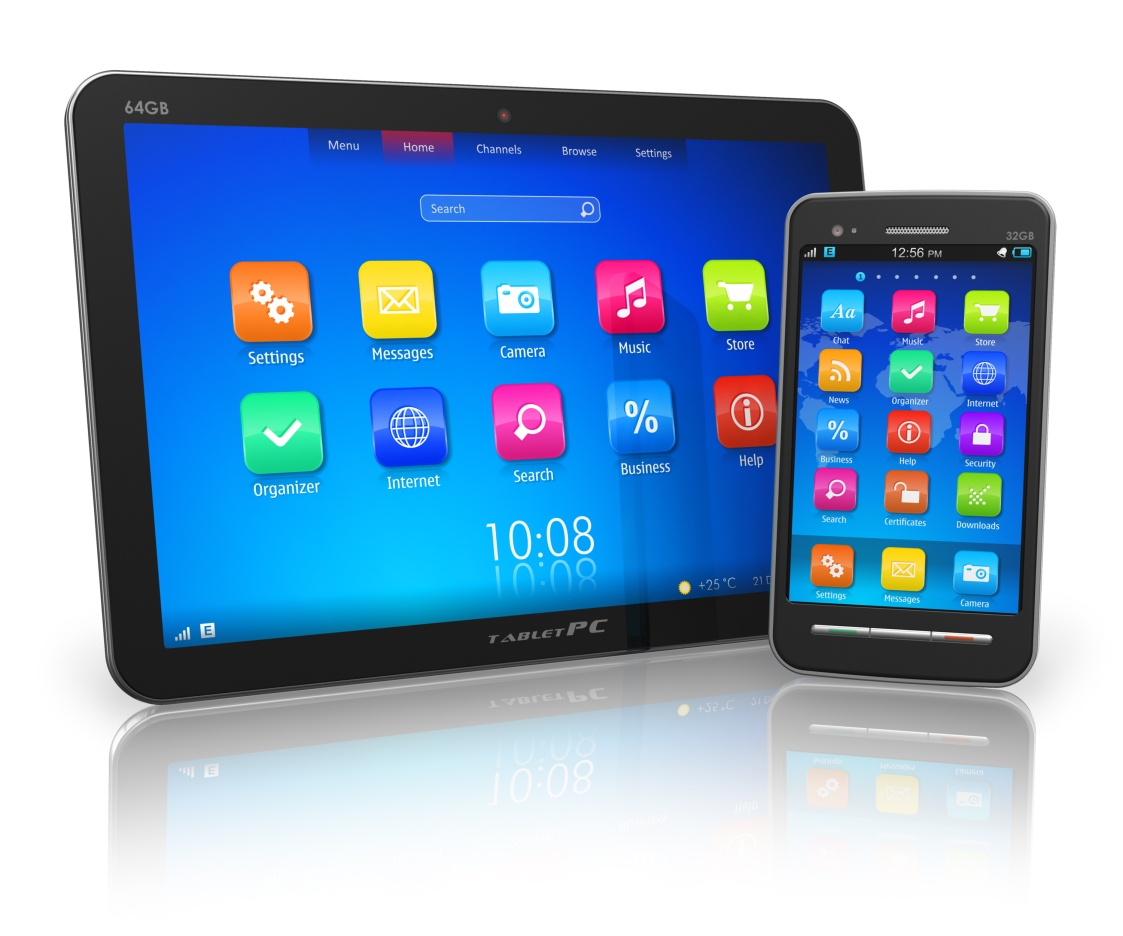
\includegraphics[width=10cm,height=10cm,keepaspectratio,scale=1.0]{Mobile_devices.jpg}
\end{figure}

\section{Motivation}

\par
Among other factors, the productivity of a programmer depends on what libraries he can have access to.
But, there are almost no rendering libraries based in ray tracing available today for mobile systems like Android, iOS or Windows 10 Mobile.
And it is likely that these systems already have enough processing power to render images with fairly complex scenes in an acceptable time by using algorithms based in ray tracing.

\par
It is also important to note that there is not much documentation about the advantages and limitations of executing different rendering algorithms in these devices.

\section{Goals}

\par
The main goal of this dissertation is to assess and demonstrate the advantages of running rendering algorithms in mobile devices.

\par
It is also intended to promote and facilitate the development of applications for mobile systems that use ray tracing techniques, with special emphasis on rendering applications.
To do this, will be developed a library that supports the fundamental operations of a ray tracing engine.
This library will allow the agile development of diverse applications, by using components that invoke the functionality of the library itself.

\par
Additionally, it is intended to supply rendering components at a higher abstraction level, like the camera, scene and the integrator that facilitates further the development of applications.

\par
Finally, it is important to do a demonstration of the rendering application with some interface layer to let the user assess the performance of several functionalities provided by the library.

\section{Document Structure}

\par
This dissertation is organized in 5 chapters: Introduction, State of the Art, Software Architecture, Demonstration: Global Illumination and Conclusion \& Future work.

\par
The first chapter describes the context and motivation behind this work, as well as its goals.
Its main purpose is to identify the problem at hand and set up goals that should be accomplished.

\par
The second chapter introduces the main concepts of ray tracing and compares different implementations of ray tracers already available in the world wide web.
The reason behind this comparison is to show how many ray tracers are already available to mobile devices and highlight the differences between the features they have.
It also provides some information about the processors of today that helps realize their ability to execute computationally demanding algorithms like ray tracing.

\par
The third chapter explains the proposed approach and explains each module developed in the library and in the rendering components.
This chapter ends with an explanation of some Android specifics, such as the user interface by characterizing its work flow and mentioning some of the challenges overcame during the development of the application.

\par
The fourth chapter summarizes the key results obtained by executing different algorithms with different number of threads and different acceleration structures.
And it will also contain a small comparison between the developed application and the Android CPU Raytracer (\cite{Android_CPU_Raytracer}).

\par
Finally, the fifth chapter ends this dissertation with the conclusions that can be withdrawn from this work and proposes some future work.

% Chapter - State of the Art ---------------------
% CHAPTER - falar de diferentes arquiteturas de ray tracing
% ou
% CHAPTER - falar de diferentes ports de apps para android
\chapter{State of the art}

\section{Ray Tracing}

\par
Ray tracing one frame can be, simultaneously, a computationally demanding task and an embarrassingly parallel task.
As tracing rays is a recursive process which aims to calculate the luminance of light of each individual pixel separately.
At least one ray is shot per pixel and in a naive approach each ray would be intersected with all the objects in the scene in order to determine which one is the closest primitive intersecting that given ray.
To evaluate the light intensity that an object scatters towards the eye, the intensity of the light reaching that object has to be evaluated as well.
Ray tracing achieves this by shooting additional secondary rays, because when a ray hits a reflecting or transparent surface, one or more secondary rays are cast from that point, simulating the reflection and refraction effects.

\begin{figure}[H]
	\centering
	\caption{Illustration of a typical ray tracer algorithm.}
	\label{Illustration of a typical ray tracer algorithm.}
	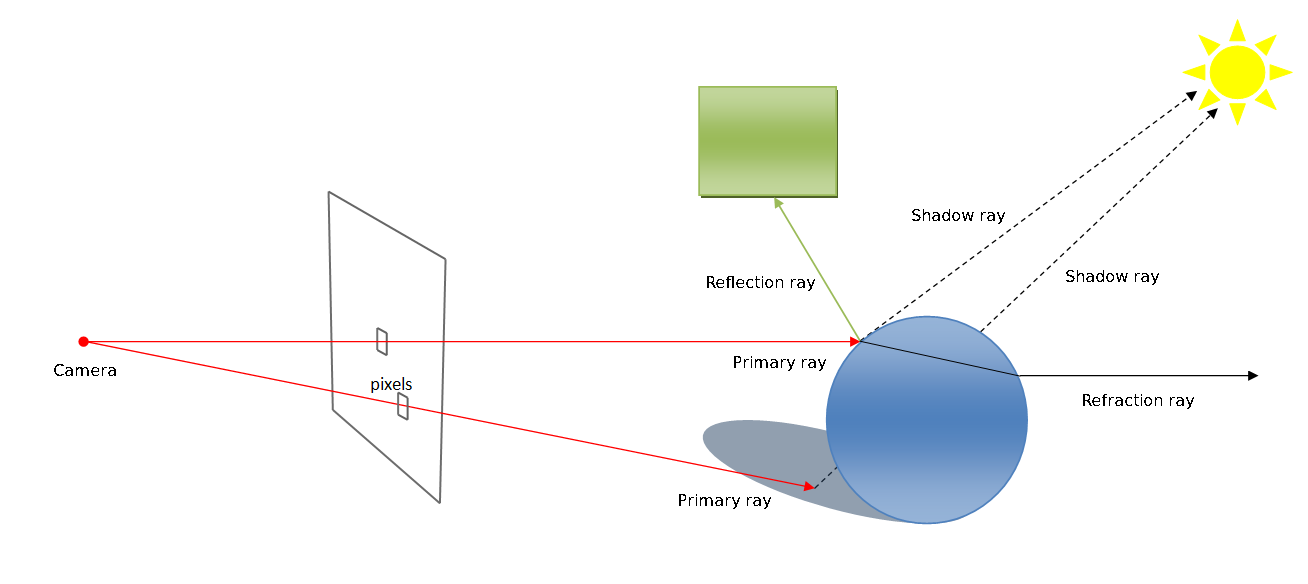
\includegraphics[keepaspectratio,scale=0.3]{Ray_Tracing.png}
\end{figure}

\par
A typical image of 1024 x 1024 pixels tends to cast at least a million primary rays and a multiple of that as shadow, reflection, refraction and secondary rays.
This is why ray tracing can't provide interactive frame rates with ease.

\section{Typical CPU features}

\par
Fortunately, the present state of available technology provides affordable machines with multiple CPU cores that can work in parallel and with great performance.
This is achieved thanks to features developed inside the processor like the cache, the multilevel pipeline, the hardware prefetching and SIMD instruction set already available in the current processors.

\par
The cache is a very small and fast multilevel memory inside the processor that temporarily stores the data read from the main memory.
This memory allows reading its content at a very low latency in the order of magnitude of around 1 nanosecond in the first level, 10 nanoseconds at second level and 50 nanoseconds at third level compared to the typical 100 nanoseconds of a DDR main memory.
The downside is that it is very small because its cost are much higher than a typical RAM memory.
Nowadays, the level 1 has 64kB, the level 2 has 256kB and the level 3 has 8 MB which is very little compared to the typical 16GB provided by the memory RAM.

\begin{figure}[H]
	\centering
	\caption{Illustration of a typical cache memory inside a microprocessor (\cite{CPU_Cache}).}
	\label{Cache.}
	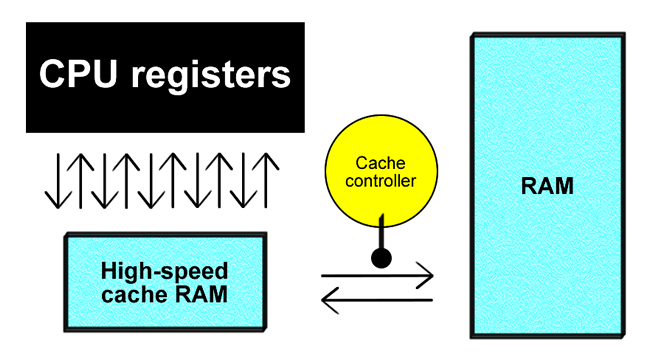
\includegraphics[keepaspectratio,scale=0.3]{cache.png}
\end{figure}

\par
The multilevel pipeline is another feature inside a processor which allows to reduce the processor's own latency by allowing a form of parallelism called instruction-level parallelism within a single processor.
Basically, one instruction is divided in some stages and it allows the possibility to execute different stages of different instructions simultaneously.
In the early days, the Classic RISC pipeline were typically divided in 5 stages:
\begin{itemize}  
	\item Fetching the instruction
	\item Decoding the instruction
	\item Executing the instruction where the arguments can be fetched from registers (1 cycle latency) or from memory (2 cycle latency)
	\item Memory access where it ensured that writing in memory was always performed in the same stage and allowed to use that value in another instruction before it was written in memory
	\item Writing back the value in the register
\end{itemize}
Nowadays, the current microprocessors have a pipeline with 8-14 stages and can be more complex than the Classic RISC, but the operating principle is the same.
This allows faster CPU throughput, which means the number of instructions that can be executed in a unit of time is greater, than it would otherwise be possible at a given clock rate.

\begin{figure}[H]
	\centering
	\caption{Illustration of the Classic RISC multilevel CPU pipeline (\cite{CPU_Pipeline}).}
	\label{Pipeline.}
	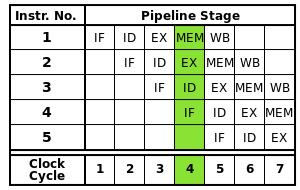
\includegraphics[keepaspectratio,scale=0.5]{Pipeline.png}
\end{figure}

\par
The hardware prefetching is, as the name implies, a feature in the processor that makes the processor fetch the data and the instructions before it really needs to execute.
This allows to reduce the time that the processor waits for the data in the main memory.

\par
Finally, SIMD instruction set is a set of special instructions that allows the processor to read or write bigger sizes of data.
Typically, a 64 bit processor can only work with 64 bits of information at a time during the execution of an instruction.
This feature can allow to read or write up to 512 bits by using special registers and additional ALUs provided in the processor.

\begin{figure}[H]
	\centering
	\caption{Illustration of a typical execution of SIMD extension (\cite{CPU_SIMD}).}
	\label{SIMD.}
	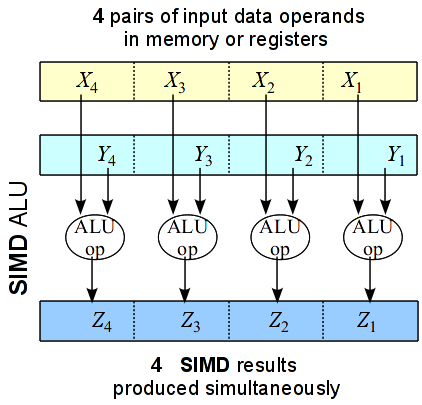
\includegraphics[keepaspectratio,scale=0.5]{SIMD.png}
\end{figure}

\par
Nowadays, even mobile devices like smart phones and tablets have multiple CPU cores with features similar to those described above.
This opens the possibility to execute more computationally demanding algorithms, like ray tracing, in these devices.

\section{Key features of Ray Tracing for this work}

\par
Ray tracing is an algorithm that can have a panoply of features or optimizations in order to reduce the time required to trace all the rays and / or to show the results as fast as possible.
It also, like any application, can have different types of software licenses and be executed in different platforms.

\par
For this work, the most important features in a ray tracer are: the type of software license, the platform where can be executed, interactivity, progressive and the type of rendering components.

\subsection{Type of software license}

\par
A software application can have different type of software license, but in order to simplify this dissertation, the software license were grouped into 3 types: Free, Commercial and Open Source.
The license Free means that the user has the right to execute freely the application but cannot copy, modify or distribute the implemented code.
The license Commercial means that the user cannot even execute the application without buying it first and cannot copy, modify or distribute the implemented code.
The license Open Source means that the user has the right to execute freely the application and can even copy, modify and distribute the implemented code.
The software license is very important in this work because it lets the user know if he can develop something over the provided software or if he can just use the application.

\subsection{Platform}

\par
An application can only be executed in the platforms that the developers compiled the code for.
So, a ray tracer that can be executed in a desktop may also or may not be executed on another platform, like a mobile device.
This information is very important in this work because it inform us whether a ray tracer can be executed in a mobile device with the typical Operating System like Android, iOS or Windows 10 Mobile.

\subsection{Interactivity}

\par
In ray tracing, interactivity means rendering an image with a very low response time, like a few milliseconds per frame.
An interactive ray tracer can render a scene with multiple frames per second.

\subsection{Progressive}

\par
A typical ray tracer shows the rendered image only after the whole process is complete.
A progressive ray tracer is a ray tracer that updates the color of pixels in the screen as soon as the rays are traced, instead of waiting for the rendering process to complete.
This means that an image is rendered quickly with some aliasing or noise and it is progressively improved over time.

\subsection{Types of Rendering Components}

\par
A ray tracer can be developed with the different rendering components programmed separately.
Some examples of rendering components are: Integrators, Cameras, Scenes, Samplers, Shapes, Lights and Accelerator Structures.
In some ray tracers, these rendering components can even be programmable by the user.
This is very important because it allows the user to develop his own renderer based in ray tracing without having to develop every feature in the ray tracer.

\section{Related work}

\par
The possibility of rendering an image with ray tracing was demonstrated in 1980 by Whitted (\cite {RT_classic}) and since then the number of libraries that provide basic ray tracing functionalities increased greatly.
There is a wide range of different ray tracers available today for the programmer to use, yet the majority can only be used with the traditional personal computer hardware (desktop or laptop).

\par
The table \ref{comparison state of the art} shows some applications or frameworks that use ray tracing available today and compares them according to their type of license, platform compatibility, interactivity, progressive and whether they allow development of your own rendering components like the integrator and sampler.
Note that some of these ray tracers provide only the engine with the basic ray tracing functions, such as creating rays and intersecting them with geometric primitives, so the rendering components are only programmable if the application that uses the engine supports it.
During the research of the available ray tracers, others than the ones presented in the table were found, but they were excluded because the documentation was very poor without explaining the basic functionalities provided or because there was no documentation at all.

\begin{table}[H]
\centering
\caption{Comparison of different applications/frameworks that use ray tracing}
\label{comparison state of the art}
\hspace*{-2.0cm}
\scriptsize
\begin{tabular}{|c|c|c|c|c|c|c|c|}
\hline
\textbf{Product}											& \textbf{License}	& \textbf{Platform}	& \textbf{Mobile}		& \textbf{Interactivity}	& \textbf{Progressive}	& \makecell{\textbf{Programmable} \\ \textbf{Components}}\\ \hline
Optix (\cite{Optix})											& F                	& Nvidia GPU 			& N				& Y                  	& Y                 		& Y\\ \hline
Optix Prime (\cite{OptixPrime})								& F                	& CPU \& Nvidia GPU 	& N				& Y                  	& Y                 		& Y\\ \hline
RenderMan RIS (\cite{RIS})									& C       	& CPU 		             & N                  		& Y                 		& Y				& Y\\ \hline
OctaneRender (\cite{OctaneRender})							& C       	& GPU 		             & N                  		& Y                 		& Y				& N\\ \hline
Embree (\cite{Embree}										& O     	& Intel CPU			& N				& Y                  	& Y                      	& Y\\ \hline
Radeon Rays (\cite{RadeonRays})							& O	& CPU \& GPU		& N				& Y                    	& Y                     	& Y\\ \hline
PBRT (\cite{PBRT})	 									& O	& CPU				& N                 		& N                 		& N				& N\\ \hline
Visionaray (\cite{Visionaray})									& O     	& CPU \& Nvidia GPU	& N                  		& Y				& Y                  	& N\\ \hline
YafaRay	(\cite{YafaRay})									& O     	& CPU 				& N                  		& N				& N                  		& N\\ \hline
tray\_rust (\cite{trayrust})									& O    	& CPU                  	& N                   	& N                  		& N                 		& N\\ \hline
micro-packet (\cite{micro-packet})							& O     	& Intel CPU 			& N                  		& N                  		& N 				& N\\ \hline
tray (\cite{tray})											& O     	& CPU 				& N				& N                     	& N                  		& N\\ \hline
The G3D Innovation Engine (\cite{G3D17})						& O	& CPU 				& N				& N                 		& N                 		& N\\ \hline
HRay (\cite{HRay})										& O     	& CPU                		& N                  		& N                      	& N				& N\\ \hline
Mitsuba (\cite{Mitsuba})										& O 	& CPU 				& N				& N                 		& N				& N\\ \hline
Indigo RT (\cite{IndigoRT})									& O 	& CPU \& GPU		& N				& Y                 		& N				& N\\ \hline
jsRayTracer (\cite{jsRayTracer})								& O 	& CPU 				& N				& Y                 		& Y				& N\\ \hline
Android CPU Raytracer (\cite{Android_CPU_Raytracer})			& O 	& CPU 				& Y (Android)		& Y                 		& N				& N\\ \hline
\end{tabular}
\normalsize
\end{table}

\subsection{Conclusions}

%Em que é que o que eu proponho é diferente das anteriores.

\par
As the table \ref{comparison state of the art} shows, there is a lack of generic ray tracing libraries for the mobile devices.
Although there are some closed-source ray tracing demo applications, only one ray tracer already available has some sort of documentation and is compatible with mobile devices, in this case with Android.
This ray tracer is open source, uses only the CPU of the device and has a good performance.
It even allows interactions with the objects during the render process.
But, it doesn’t support progressive rendering and also does not allow the programmers to use their own rendering components.

\par
This dissertation aims to fix this lack of libraries, by providing one that contains ray tracing basic functionalities and the ability to let the programmer be able to develop their own rendering components like the sampler, integrator, camera and shapes of virtual objects.
It also studies the drawbacks that these mobile devices may have comparing with the average multi-core personal computer hardware.
And finally, a small comparison was made with the Android CPU Raytracer (\cite{Android_CPU_Raytracer}) in order to illustrate the advantages and disadvantages of both.
This comparison is important because it enriches all the work done, as it demonstrates if the performance of the provided features are relatively efficient.

% Chapter - Ray Tracing -------------------------
% CHAPTER - explicar a implementaçao da lib
% CHAPTER - explicar a implementaçao dos componentes
\chapter{Software architecture}

\section{Approach}

\par
The development of this demonstration application involves the distinction of three layers of abstraction: user interface, rendering components and the library itself.

\par
The top layer is the User Interface which is obviously application, and eventually device, dependent.
The user interface of this dissertation's demo application is very simple and just allows the user to see the rendered image and choose some rendering components to use, like the integrator, the sampler, the number of threads and samples and choose the scene to render.
Although this layer is useful, this dissertation focuses only on the middle and bottom layers.

\begin{figure}[H]
	\centering
	\caption{Illustration of the developed User Interface.}
	\label{UI.}
	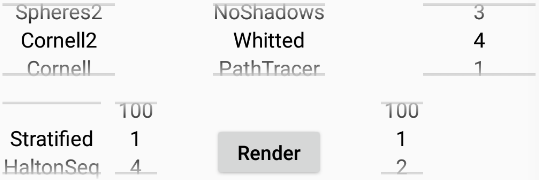
\includegraphics[width=10cm,height=10cm,keepaspectratio,scale=1.0]{UI.png}
\end{figure}

\par
The middle layer provides the rendering components which are abstracted concepts about rendering that use functionalities that the library offers to the programmer.
Some of these rendering components are the camera, the light, the sampler and the integrator.
These rendering components are useful for the programmer since it allows them to use features without having the need to know how these were developed.
And, of course, this facilitates and accelerates the development of new rendering applications.

\par
Lastly, the bottom layer is the library itself, which contains the business logic of basic features in a renderer, that the rendering components use.
These features are basic functionalities of a ray tracer engine like: create vectors and points, create different primitives with different materials, cast rays and intersect rays with the primitives.

\par
It is also important to mention that the demo application was developed in order to show the developed features, the performance achieved in the mobile devices and also to help promote the library.
This demo application is a good way to test it in several Android devices like a smart phone or a tablet.

\begin{figure}[H]
	\centering
	\caption{Illustration of the 3 layers in the application}
	\label{Illustration of the 3 layers in the application}
	\includegraphics[width=10cm,height=10cm,keepaspectratio,scale=1.0]{Layers.png}
\end{figure}

\par
Besides the abstraction layers, there are some important strategic decisions made in order to guide the progress of the development of this library.

\par
The first decision was: the primary rays always have origin in the camera.
This decision was made in order to not mix the code of the integrator with the ray tracer renderer engine.

\par
Other decision made was to make the rendering process progressive, which means that the rendered image is incrementally refined with more and more traced rays.
As the integrator will be converging to better values.
This is important in order to give the user a fast rendered image, with some noise or aliasing, and converge it progressively to a better solution with higher details and practically without any visual noise or aliasing.

\par
Another thought aspect that was studied is the permission of dynamic scenes and / or dynamic cameras, which means to let the programmer modify the camera or the scene while the ray tracer is rendering it.
This makes possible to build challenging applications and also provide more interesting scenes and more eye candy applications for the final user.

\par
Last, but not least, is that the code was developed in a modular way, in this case was programmed in an object oriented manner.
This allows the programmers to code their own rendering components, like the integrator, camera, sampler and light, without having to develop the basic features in the renderer engine.

\section{Methodology}

\par
In order to take advantage of most of the mobile CPU resources and give a good performance for the applications, the library and the rendering components were developed using the native programming language C++.
This was achieved by using the Native Development Kit (NDK) provided by the Integrated Development Environment (IDE) Android Studio.
The User Interface was developed in Java using the traditional Software Development Kit (SDK) provided by the Android Studio because there is no framework in the NDK that helps the programmer design his own user interface.
Despite that, its performance is not very important because it doesn't interfere significantly with the others layers of the application.



\iffalse

\section{Work plan}

\par
The development of this dissertation will be done in six stages.

\par
The first stage involves the survey of state of the art about ray tracers built for mobile systems, in order to understand the capacities and limitations of these devices when running rendering algorithms.

\par
The second stage is to make the requirements specification in order to:

\begin{itemize}
\item Describe the functionalities of the library.
\item Explain how the user interact with the external interfaces.
\item Demonstrate the design constraints imposed on an implementation of a custom rendering component.
\end{itemize}

\par
The third stage will address the development of the architecture of the entire system.
The study performed in the previous stages will serve as the basis for this development, where this architecture should be able to address all the possible problems that might arise in the development process.

\par
The fourth stage will be the development and test of the software, where it should be relatively quick if the previous stage was done properly.

\par
Next it will be made a demo application in order to illustrate the possibilities and limitations of this rendering process in the mobile devices.

\par
Finally, the writing of this dissertation will be done throughout the entire project, but there will be a reinforced effort at the end along with the writing of an article.

\par
In short, the work plan of this dissertation should be as follows:

\begin{enumerate}

\item Survey of the State of the Art (2 weeks)
\item Requirements specification (2 weeks)
\item Development of Software Architecture (3 months)
\item Development and test of the library (2 weeks)
\item Development of a demonstration (2 weeks)
\item Writing the dissertation and an article (1 month)

\end{enumerate}

\begin{table}[H]
\centering
\caption{Scheduling for this dissertation}
\label{Scheduling for this dissertation}
\begin{tabular}{|c|c|c|c|c|c|c|}[H]
\hline
\textbf{}                               & \multicolumn{6}{c|}{\textbf{2017}} \\ \hline
                                        & Jan  & Feb & Mar & Apr & May & Jun \\ \hline
Survey of the State of the Art          & X    &     &     &     &     &     \\ \hline
Requirements specification              & X    &     &     &     &     &     \\ \hline
Development of Software Architecture    &      & X   & X   & X   &     &     \\ \hline
Development and test of the library     &      &     &     &     & X   &     \\ \hline
Development of a demonstration          &      &     &     &     & X   &     \\ \hline
Writing the dissertation and an article &      &     &     &     &     & X   \\ \hline
\end{tabular}
\end{table}

\fi



\section{Library}

\par
As stated above, this library was implemented in an object-oriented fashion.
The most important classes that provide functionalities already developed for the user to use are:

\begin{itemize}
\item Renderer: class that starts the rendering process and stores the calculated pixels colors in a C style array.
\item Scene: class that stores the geometry information in vectors and provides methods to trace rays in the scene without any acceleration structures.
\item Shapes: set of classes that allows to create triangles, spheres and planes.
\item Material: class that stores all 4 types of material color:
\begin{itemize}
	\item Emission light color
	\item Diffuse reflection color
	\item Specular reflection color
	\item Specular refraction color
\end{itemize}
\item Primitive: class that stores the shape and material of each primitive in the scene.
\item Ray: class that represents a ray casted into the scene.
\end{itemize}

\subsection{Third parties dependencies}

\par
Before describing each functionality provided in each class developed, it is important to mention that this library uses 3 other libraries developed in C++ by third parties.
Those libraries are:

\begin{itemize}
	\item OpenGL Mathematics (\cite{GLM}): used to create 3d points and vectors, perform geometry calculations and store pixels and primitives colors.
	\item tinyobjloader (\cite{tinyobjloader}): used to load scenes from wavefront obj files.
	\item Google Test (\cite{GoogleTest}): used to create some unit tests and to mock some classes.
\end{itemize}

\par
All these libraries are Android compatible and are reliable in terms of performance and maintenance.

\par
Besides being dependent on these 3 libraries, this library also depends on OpenGL ES 2.0 (\cite{OpenGL_ES_2}) from Android SDK and depends on CMake (\cite{CMake}) in order to compile the application.

\subsection{Renderer}

\par
The Renderer is the closest class to the application that starts the rendering process.
This class provides two main methods:
\begin{lstlisting}
void renderFrame(::std::uint32_t *bitmap, ::std::int32_t numThreads, ::std::uint32_t stride) noexcept;
void stopRender() noexcept;
\end{lstlisting}

\par
The \textit{renderFrame} method starts the rendering process and writes the calculated light luminance of each pixel in the parameter \textit{bitmap}.
This method also allows to choose the number of threads that will render the image into the bitmap, and needs the stride of that bitmap array.
The image plane is divided into 16 tiles of pixels and it is traced one primary ray per pixel in each tile.

\begin{figure}[H]
	\centering
	\caption{Illustration of tiling the image plane.}
	\label{Illustration of tiling the image plane.}
	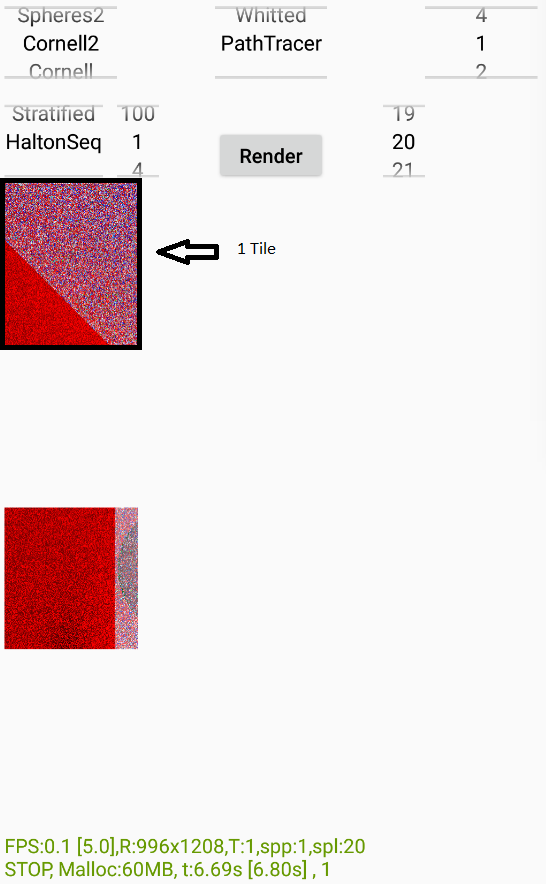
\includegraphics[width=10cm,height=10cm,keepaspectratio,scale=1.0]{tiling.png}
\end{figure}

\par
The \textit{stopRender} method only serves to stop the rendering process without cleaning the pixels' colors already calculated.

\subsection{Scene}

\par
The Scene is the class that handles the process of intersecting a ray with the primitives and source lights in the scene.
Besides providing a vector to add the light sources and a vector to add primitives to the scene, it also provides two main methods:
\begin{lstlisting}
Intersection trace(Intersection intersection, const Ray &ray) noexcept;
Intersection shadowTrace(Intersection intersection, const Ray &ray) noexcept;
\end{lstlisting}

\par
The \textit{trace}, as the name implies, is a method that tries to intersect a ray with all the primitives and light sources in the scene.
And It returns the closest intersection to the origin of that ray.
This method is used to determine the intersection of the casted ray with the primitives in the scene.

\par
The \textit{shadowTrace}, is similar to the \textit{trace} method but with the difference that returns the first intersection found.
The purpose of this method is to simulate the shadows in the scene, like it is illustrated in figure \ref{Illustration of shadow rays casting.}.

\begin{figure}[H]
	\centering
	\caption{Illustration of shadow rays casting (\cite{ShadowRays}).}
	\label{Illustration of shadow rays casting.}
	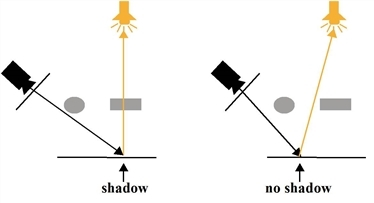
\includegraphics[width=10cm,height=10cm,keepaspectratio,scale=1.0]{Shadow_Ray.jpg}
\end{figure}


\subsection{Shapes}

\par
In order to make possible to generate scenes with all kind of objects, it was developed 3 types of shapes: plane, sphere and triangle.
All shapes provide only one method:
\begin{lstlisting}
Intersection intersect(const Intersection &intersection, const Ray &ray) const noexcept;
\end{lstlisting}
This method determines if a ray intersects the shape and returns the intersection.
It is important to mention that, obviously, each shape was developed with different algorithm.

\subsubsection{Plane}

\par
The plane is an essential primitive shape because it allows the user to build indoor scenes.

\par
The construction of a plane requires just an arbitrary point in the plane and the normal of the plane.
So, the intersect method implemented has the following algorithm:

\begin{lstlisting}
projection = planeNormal . rayDirection
if (|projection| <= 0) return false
distance = planeNormal . (planePoint - rayOrigin) / projection
if (distance <= 0 || distance > rayMaxDistance) return false
intersectionPoint = rayOrigin + rayDirection * distance
return Intersection(intersectionPoint, planeNormal, material)
\end{lstlisting}


\begin{figure}[H]
	\centering
	\caption{Illustration of a ray intersecting a plane (\cite{PlaneRayIntersection}).}
	\label{Plane.}
	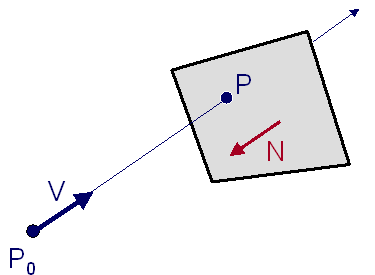
\includegraphics[keepaspectratio,scale=0.4]{RayToPlane.png}
\end{figure}

\subsubsection{Sphere}

\par
The sphere is also an important primitive shape because it allows the user to build some common objects with a shape of a ball.

\par
The construction of a sphere requires just the point in the center and the radius of the sphere.
It also should be noted that a ray can intersect a sphere at two points and therefore it is necessary to determine the closest intersection point to the origin of the ray.
So, the intersect method implemented has the following algorithm:

\begin{lstlisting}
centerToOrigin = rayOrigin - sphereCenter
B = 2 * centerToOrigin . rayDirection
C = centerToOrigin.magnitude - radius
disciminant = B^2 - 4*C
if (discriminant <= 0) return false
distance1 = (-B + sqrt{discriminant} * 0.5)
distance2 = (-B - sqrt{discriminant} * 0.5)
distance = min(distance1, distance2)
if (distance <= 0 || distance > rayMaxDistance) return false
intersectionPoint = rayOrigin + rayDirection * distance
sphereNormal = intersectionPoint - sphereCenter
return Intersection(intersectionPoint, sphereNormal, material)
\end{lstlisting}

\begin{figure}[H]
	\centering
	\caption{Illustration of a ray intersecting a sphere in two points (\cite{SphereRayIntersection}).}
	\label{Sphere.}
	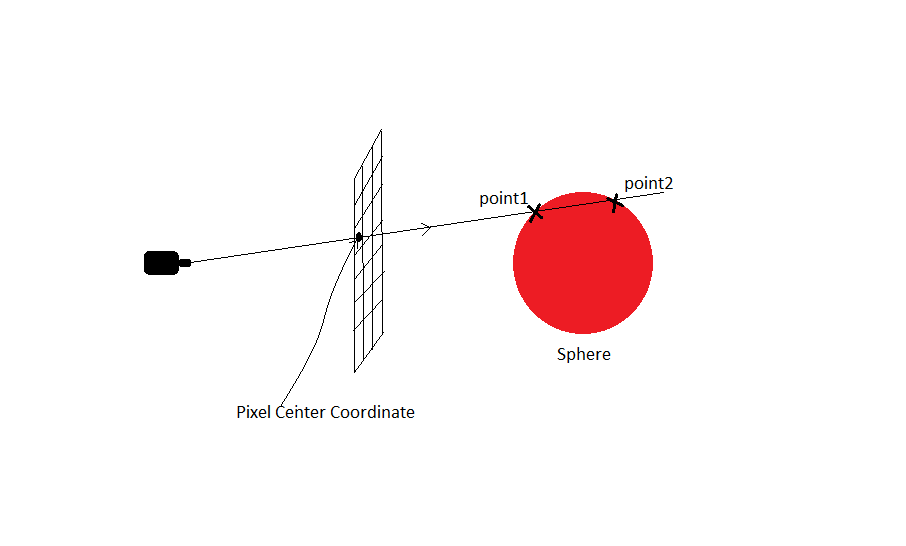
\includegraphics[keepaspectratio,scale=0.4]{Ray_Sphere_Intersection.png}
\end{figure}

\subsubsection{Triangle}

\par
And finally, obviously the triangle has also been implemented because, as it is the simplest primitive with an area, it allows to build many different object shapes.

\par
The construction of a triangle requires three points
$[A, B, C]$
, two vectors
$[AB, AC]$
and the normal of the triangle.
So, the intersect method implemented has the following algorithm:

\begin{lstlisting}
perpendicularVector = rayDirection x AC
projection = AB . perpendicularVector
if(|projection| <= 0) return false
vectorToRay = rayOrigin - A
u = (vectorToRay . perpendicularVector) / projection
if (u < 0 || u > 1) return false
perpendicularVector2 = vectorToRay x AB
v = (rayDirection . perpendicularVector2) / projection
if(v < 0 || (u + v) > 1) return false
distance = (AC . perpendicularVector2) / projection
intersectionPoint = rayOrigin + rayDirection * distance
return Intersection(intersectionPoint, triangleNormal, material)
\end{lstlisting}

\begin{figure}[H]
	\centering
	\caption{Illustration of a ray intersecting a triangle (\cite{TriangleRayIntersection}).}
	\label{Sphere.}
	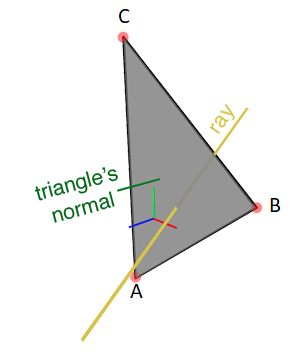
\includegraphics[keepaspectratio,scale=1.0]{triangle.png}
\end{figure}

\subsection{Acceleration Structures}

\par
As previously stated, the rendering algorithms based on ray tracing can be very computationally demanding, like Path Tracing and Bidirectional Path Tracing.
These algorithms are very computationally demanding because 
Luckly, there are already known techniques that helps to acc

\subsubsection{Regular Grid}

\par
Regular Grid ...

\subsubsection{Bounding Volume Hierarchy}

\par
Bounding Volume Hierarchy ...

\section{Rendering Components}

\par
In order to show the functionalities provided by the library, it was developed a few Rendering Components.
It is provided the perspective camera, an area light and point light, four Samplers and three Shaders.

\subsection{Shaders}

\par
The implemented ray tracer was programmed objected oriented, so each Rendering Component was developed separately.
This allows the user to develop his own Rendering Components without having to develop the ray tracer engine.

\par
In this context, a shader is the Rendering Component that describes how the Rendering Equation is approximated.
The Rendering Equation describes how the total radiance reflected by any point
$p$
of a surface in a direction
$\omega$$r$
is calculated.
The Bidirectional Reflectance Distribution Function (BRDF) is a function that tries to approximate the Rendering Equation.
In summary, a shader, in this context, is the algorithm of a BRDF.

\begin{figure}[H]
	\centering
	\caption{Illustration of the rendering equation describing the total amount of light emitted from a point
	$x$
	along a particular viewing direction and given a function for incoming light and a BRDF.}
	\label{Rendering_Equation.}
	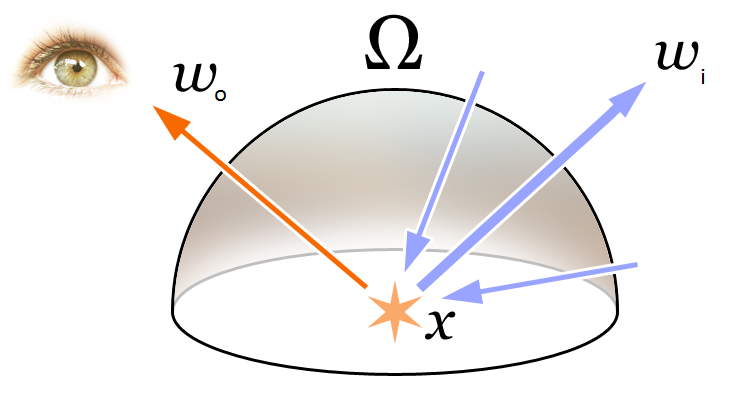
\includegraphics[width=10cm,height=10cm,keepaspectratio,scale=1.0]{Rendering_eq.png}
\end{figure}

\par
There was developed three shaders: NoShadows, Whitted and PathTracer.
All shaders provide only one main method that allows the user to calculate the RGB color of a pixel with the information of a ray and the respective intersection.

\begin{lstlisting}
void shade(RGB &rgb, Intersection &intersection, Ray &ray) const override;
\end{lstlisting}

\par
The parameter
$rgb$
is where the color of the pixel will be calculated and the
$intersection$
contains the necessary information about the intersection of a ray with the primitive like the intersection point, its normal and the material of the intersected material.
Finally the parameter
$ray$
is where the information about the ray like the origin of the ray and its direction is accessed.

\subsubsection{NoShadows}

\par
NoShadows is the simplest shader because, as the name implies, it does not synthesize the shadows and it only simulates the direct lighting.
This BRDF only simulates direct lighting in primitives with diffuse surfaces and it does not take into account the light coming from other points.
As already said, the indirect lighting is not fully simulated but rather simplified in a way of fixed ambient light of about 10\% of the color of the objects.

\par
The algorithm developed is as following:

\begin{lstlisting}
if (intersected material is diffuse) {
  for each light source
  	for each sample
	    vectorToLight = lightPosition - intersectionPoint
	    cos_N_L = vectorToLight . intersectionNormal
	    if (cos_N_L > 0) rgb += kD * radLight * cos_N_L
  rgb /= #samples
  rgb /= #lights
  rgb += kD * 0.1 //Ambient light
}
\end{lstlisting}

\begin{figure}[H]
	\centering
	\caption{NoShadows shader.}
	\label{NoShadows shader.}
	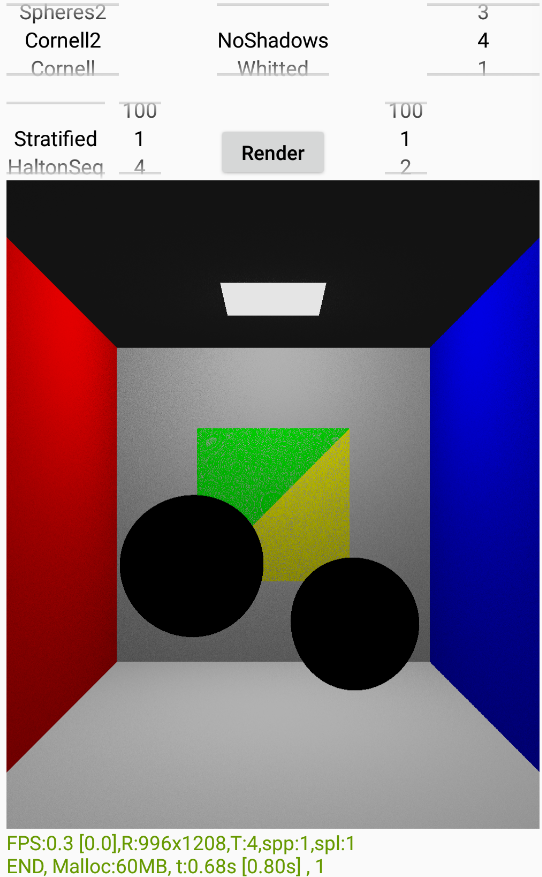
\includegraphics[keepaspectratio,scale=0.3]{NoShadows.png}
\end{figure}

\subsubsection{Whitted}

\par
As the name of this shader implies, Whitted is the algorithm demonstrated by Whitted in 1980s.
Like the previous shader, it doesn't simulate indirect lighting.
This BRDF calculates the reflected light on diffuse and specular surfaces, as well as the light refracted on surfaces with a degree of transmission, such as water.
In order to simulate a reflective and refractive surfaces, the algorithm was divided into each case.
This makes it possible to simulate refractive surfaces, reflective surfaces and even refractive and reflective surfaces.

\par
The reflected light in a diffuse surface is calculated by adding the casting rays in direction to the lights.
These rays are called shadow rays and their radiance are multiplied by the dot product between vector to the light and the shading normal.
At the end, the summation is multiplied by the diffuse color of the intersected primitive and divided by the number of samples taken.

\par
The reflected light in a specular surface is calculated in a different way.
The specular ray is casted and ray traced, then the obtained radiance is multiplied by the specular color of the intersected primitive.
The reflection direction is the subtraction between the double of dot product between the inverse of the ray direction and the shading normal multiplying by the shading normal, and the inverse of the ray direction.

\begin{figure}[H]
	\centering
	\caption{Reflections projected on the floor and on the spheres.}
	\label{Reflection.}
	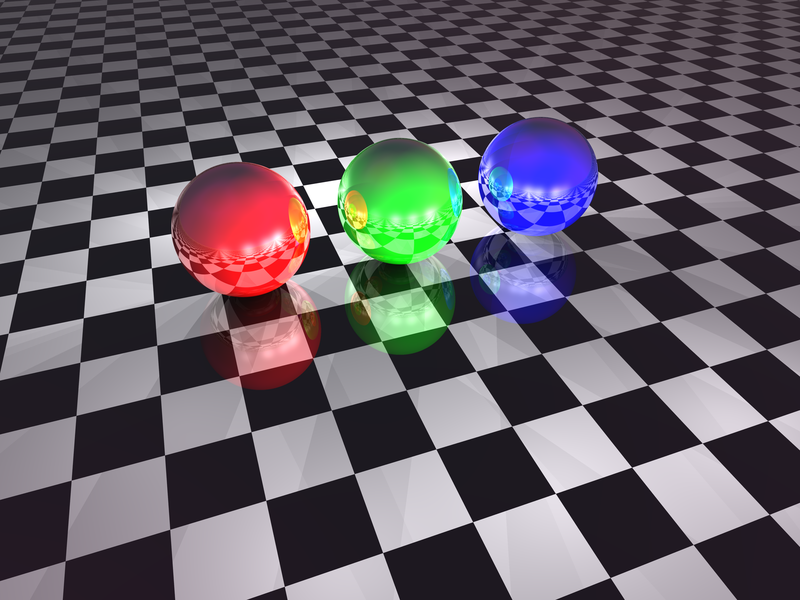
\includegraphics[keepaspectratio,scale=0.3]{Reflection.png}
\end{figure}

\par
Finally, the refracted light in a transmission surface is calculated by using the refractive index of the intersected primitive and the ray direction and shading normal.
First, the shading normal is inverted if the origin of the ray was inside a primitive, like a sphere, and if it was not then the refractive index is inverted.
Then, it is calculated two auxiliary scalar projections:
$cosTheta1$
and
$cosTheta2$
.
$cosTheta1$
is the dot product of the inverse of the shading normal and the ray direction, and
$cosTheta2$
is the difference of 1 and refractive index squared multiplied by one minus
$cosTheta1$
squared.
Then, if
$cosTheta2$
is greater than zero, then the direction of the transmission ray is ray direction multiplied with refractive index plus shading normal multiplied by refractive index multiplied $cosTheta1$
minus square root of 
$cosTheta2$
.
Else, the direction of the transmission ray is just ray direction plus shading normal multiplied by the double of
$cosTheta1$
.
And, as usual, the transmission ray is traced and its radiance is multiplied by the transmission component of the intersected primitive.

\begin{figure}[H]
	\centering
	\caption{Refraction of light at the interface of two media of different refractive indices.}
	\label{Refraction.}
	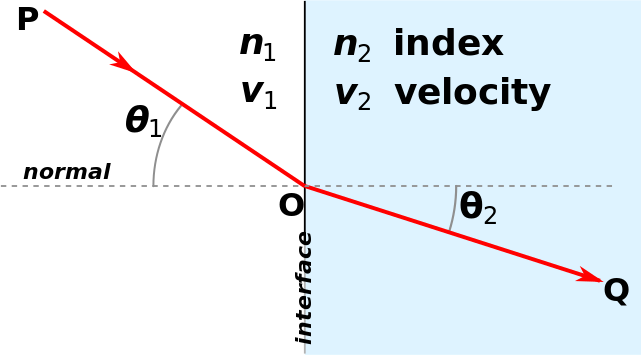
\includegraphics[keepaspectratio,scale=0.3]{Refraction.png}
\end{figure}

\par
The algorithm developed is as following:

\begin{lstlisting}
if (intersected material is diffuse) {
  for each light source
    for each sample
      vectorToLight = lightPosition - intersectionPoint
      cos_N_L = vectorToLight . shadingNormal
      if (cos_N_L > 0) {
        Ray shadowRay(intersectionPoint, vectorToLight, distanceToLight, rayDepth + 1)
        if (!shadowTrace(shadowRay)) rgb += radLight * cos_N_L
      }
  rgb *= kD
  rgb /= #samples
}

if (intersected material is specular reflective) {
  reflectionDir = (2 * symRayDirection . normal) * normal - symRayDirection
  Ray specularRay(intersectionPoint, reflectionDir, rayDepth + 1)
  rgb += rayTrace (specularRay) * kS
}

if (intersected material is specular refractive) {
  if (shadingNormal . rayDirection > 0) {
    //we are inside the medium
    shadingNormalT = -1 * shadingNormal
    n = 1 / n
  }
  n = 1 / n
  cosTheta1 = -shadingNormalT . rayDirection
  cosTheta2 = 1 - n^2*(1-cosTheta1^2)
  if (cosTheta2 > 0)
    transmissionRay.dir = ((rayDir*n) + (shadingNormalT*(n*cost1 - sqrt(cost2))))
  else
    transmissionRay.dir = (rayDir + shadingNormalT*(cost1 * 2))
  rgb += rayTrace(transmissionRay) * kT
}
\end{lstlisting}

\begin{figure}[H]
	\centering
	\caption{Whitted shader.}
	\label{Whitted shader.}
	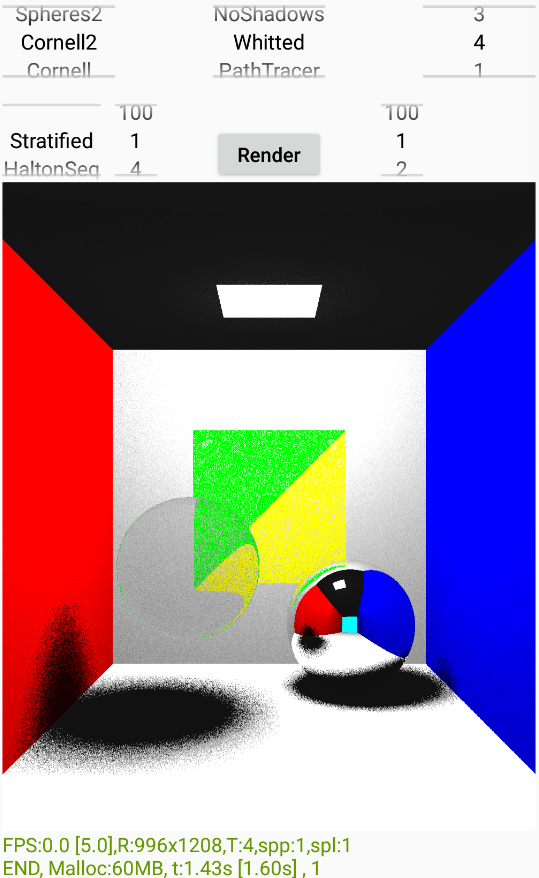
\includegraphics[keepaspectratio,scale=0.3]{Whitted.png}
\end{figure}


\subsubsection{PathTracer}

\par
Finally, the last shader developed is the canon Path Tracer.
Unlike the previous shaders, this one fully simulates both direct and indirect lighting.
But, like the previous shader, this algorithm simulates the light reflected on diffuse and specular surfaces, as well as the light refracted on transparent primitives.

\par
The light reflected on diffuse surfaces is divided in two parts: direct lighting and indirect lighting.
The direct lighting is calculated in a similar way to the Whitted shader but with the difference that samples are not taken from all sources of light but rather only one.
The light source in each sample is chosen randomly.
Then the obtained light radiance is multiplied by the Probability Density Function (PDF) in order to approximate the expected value.
In this case the PDF is as simple as
$1 / \#lights$.

\par
Finally, the indirect lighting reflected in diffuse surfaces is calculated in a much more complex way.
First it is generated, from the intersected point, a random direction on an unit hemisphere with a PDF proportional to cosine-weighted solid angle
($PDF: p(\Theta) = cos\theta / \pi$,
$x = cos(2\pi r1)\sqrt{1-r2}$,
$y = sin(2\pi r1)\sqrt{1-r2}$,
$z = \sqrt{r2}$)
.
This kind of PDF is one of the best ways to render images with path tracing that the rendering equation converges to the expected value as fast as possible.
Then a rotation matrix is built, where it lets rotate a vector around an arbitrary axis with a given angle.

\begin{figure}[H]
	\centering
	\caption{Rotation matrix from an arbitrary axis and an angle.}
	\label{Rotation_matrix.}
	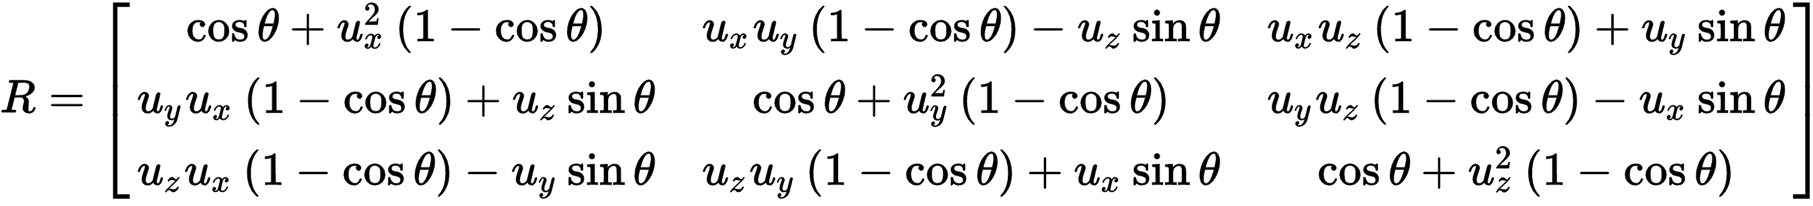
\includegraphics[keepaspectratio,scale=0.5]{Rotation_Matrix.png}
\end{figure}

Then the proper coordinates in the world view is just: $globalCoordinates = localCoordinates * rotationMatrix$.
And the indirect lighting on diffuse surfaces is then the multiplication of the ray traced light radiance with the color of the primitive and
$\pi$
, and divided by the probability of stopping the Russian roulette.

\par
The reflected light in a specular surface and the refracted light are simulated in a similar way to the Whitted algorithm presented previously.

\par
The algorithm developed is as following:

\begin{lstlisting}
if (intersected material is diffuse) {
  for each light
    for each sample
      light = samplerLight.getSample()
      vectorToLight = lightPosition - intersectionPoint
      cos_N_L = vectorToLight . shadingNormal
      if (cos_N_L > 0) {
        Ray shadowRay(intersectionPoint, vectorToLight, distanceToLight, rayDepth + 1)
        if (!shadowTrace(shadowRay)) rgb += radLight * cos_N_L
      }
  rgb *= kD
  rgb *= #lights
  rgb /= #samples

  if (rayDepth <= RAY_DEPTH_MIN || uniform_dist(gen) > finish_probability) {
    local = Generate random direction on unit hemisphere 
    proportional to cosine-weighted solid angle

    RotationMatrix = Rotation matrix from axis and angle

    Vector3D up = (0,1,0)
    Vector3D u = intersectionNormal x up
    if (u == 0) u.x = 1
    cosTheta = up . intersectionNormal
    sinTheta = 1 - cosTheta^2
    if (sinTheta < 0) sinTheta *= -1
    sinTheta = sqrt(sinTheta)

    global = local * rotationMatrix

    Ray secundaryRay (globalX, globalY, globalZ, intersectionPoint, rayDepth + 1)

    LiD = rayTrace(secundaryRay) * kD * PI

    if (rayDepth > RAY_DEPTH_MIN) LiD /= continue_probability
    if(secundaryRay intersects light) LiD = 0

    rgb += LiD
  }

}

if (intersected material is specular reflective) {
  reflectionDir = (2 * symRayDirection . normal) * normal - symRayDirection
  Ray specularRay(intersectionPoint, reflectionDir, rayDepth + 1)
  rgb += rayTrace (specularRay) * kS
}

if (intersected material is specular refractive) {
  if (shadingNormal . rayDirection > 0) {
    //we are inside the medium
    shadingNormalT = -1 * shadingNormal
    n = 1 / n
  }
  n = 1 / n

  cosTheta1 = -shadingNormalT . rayDirection
  cosTheta2 = 1 - n^2*(1-cosTheta1^2)

  if (cosTheta2 > 0)
    transmissionRay.dir = ((rayDir*n) + (shadingNormalT*(n*cosTheta1 - sqrt(cosTheta2))))
  else
    transmissionRay.dir = (rayDir + shadingNormalT*(cosTheta1 * 2))

  rgb += rayTrace(transmissionRay) * kT
}
\end{lstlisting}

\begin{figure}[H]
	\centering
	\caption{PathTracer shader.}
	\label{PathTracer shader.}
	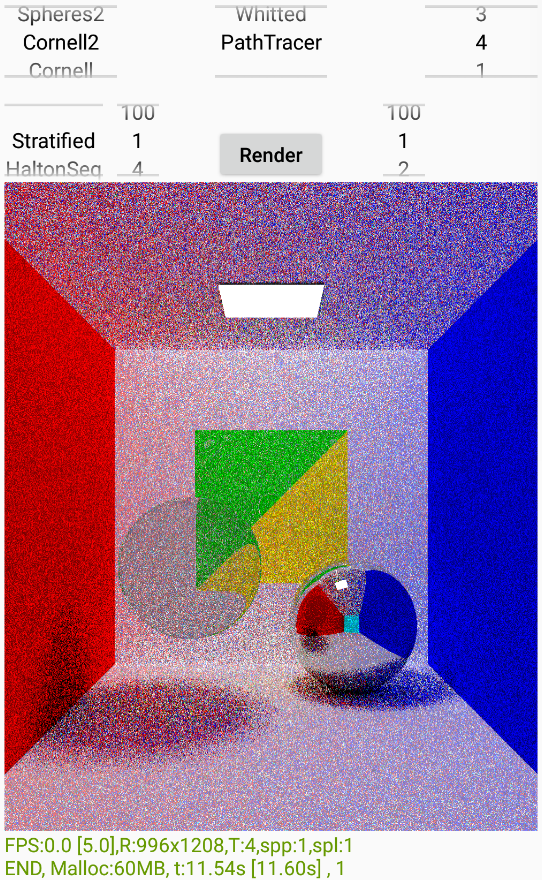
\includegraphics[keepaspectratio,scale=0.3]{PathTracer.png}
\end{figure}


\subsection{Samplers}

\par
There were implemented four samplers: Constant, Stratified, HaltonSequence and Random.

\par
All samplers just provide one method for the user to use:
\begin{lstlisting}
float getSample(const unsigned int sample);
\end{lstlisting}

\par
The
$getSample$
method receives as parameter the number of the current sampler and returns the the actual sample.
An atomic variable
$sample$
is used to count the current index of the samples.

\subsubsection{Constant}

\par
This sampler is the simplest because it always returns the same number passed to the constructor.

\par
The algorithm of the
$getSample$
is just:

\begin{lstlisting}
return value
\end{lstlisting}


\subsubsection{Stratified}

\par
This sampler makes each sample at equal distance
$(1 / domainSize)$
and in ascending order.
For example, for a domain size of 4, the samples taken are going to be: 0, 0.25, 0.5 and 0.75.

\par
The algorithm of the
$getSample$
is then:

\begin{lstlisting}
//atomic operation
current = sample++
if (current >= (domainSize * (sampleParam + 1))) {
  sample--
  return 1
}
task = current - (sampleParam * domainSize)
return task / domainSize
\end{lstlisting}


\subsubsection{HaltonSequence}

\par
As the name implies, this sampler generates the Halton sequence.

\par
Halton sequence is a quasi random number sequence which is a deterministic sequence with low discrepancy.

These sequences are usually good for Rendering Algorithms like Path Tracing because it can make the rendering equation converge faster (with fewer samples).

\begin{figure}[H]
	\centering
	\caption{Halton sequence in a 2D image plane.}
	\label{Halton_sequence_2D.}
	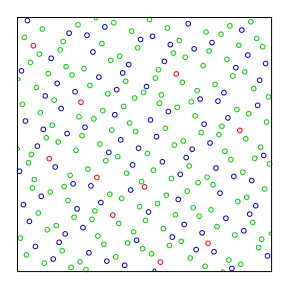
\includegraphics[keepaspectratio,scale=0.5]{Halton_sequence_2D.png}
\end{figure}

\par
The algorithm of the
$getSample$
is as following:

\begin{lstlisting}
//atomic operation
current = sample++
if (current >= (domainSize * (sampleParam + 1))) {
  sample--
  return 1
}
task = current - (sampleParam * domainSize)

f = 1
result = 0
while (task > 0) {
  f = f / base
  result = result + f * (index % base)
  task = floor(index / base)
}
return result
\end{lstlisting}

\subsubsection{Random}

\par
This sampler is just a wrapper to call the function rand() of the standard C library.

This function is a pseudo random number generator (PRNG), which is an algorithm for generating a sequence of numbers whose properties approximate the properties of sequences of random numbers.
Although the PRNG-generated sequence is not truly random, because it is completely determined by an initial value, called the PRNG's seed.
These sequences are usually used in simulations that use Monte Carlo methods like the Monte Carlo Ray Tracing.

\begin{figure}[H]
	\centering
	\caption{Pseudorandom sequence in a 2D image plane.}
	\label{Pseudorandom_sequence_2D.}
	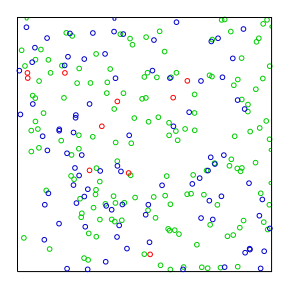
\includegraphics[keepaspectratio,scale=0.5]{Pseudorandom_sequence_2D.png}
\end{figure}

\par
So the algorithm of the
$getSample$
is just:

\begin{lstlisting}
return rand() / RAND_MAX
\end{lstlisting}


\subsection{Lights}

\par
There were implemented two types of light sources: PointLight and AreaLight.
These light sources provide the user two main methods:

\begin{lstlisting}
const Point3D getPosition(void);
bool intersect(Intersection &intersection, const Ray &ray, const Material &) const;
\end{lstlisting}

\par
The
$getPosition$
method just returns the position of the light source and the 
$intersect$
method determines whether a given
$ray$
as a parameter intersects this light source and, if it intersects, writes the result to the
$intersection$
parameter.

\subsubsection{PointLight}

\par
The PointLight is the simplest form of a light because, as the name implies, is just a point of light.

\par
Therefore, the
$getPosition$
method is very simple because it only returns the position of the light source determined in its constructor:

\begin{lstlisting}
return position;
\end{lstlisting}

\par
And the
$intersect$
method is also quite simple because it always returns false.
This is because the probability of a ray intersecting a single 3D point in the world is practically nil.

\subsubsection{AreaLight}

\par
The AreaLight implemented has a shape of a triangle.
This shape is intended as it allows to generate a random point in a triangle with barycentric coordinates.

\par
A triangle with 3 points: A, B and C.
We get vectors AB and AC, being:

\begin{lstlisting}
AB=[Bx-Ax,By-Ay,Bz-Az] and AC=[Cx-Ax,Cy-Ay,Cz-Az].
\end{lstlisting}

\par
These vectors tell how to get from point A to the other two points in the triangle, by telling us what direction to go and how far.
So, with barycentric coordinates R=1/3, S=1/3 and T=1/3, we get the point in the center of the triangle.
To generate a random point in the triangle, we have to generate 2 random numbers between 0 and 1 (R and S).
Then we have to make sure we stay inside the triangle by checking if they are larger than one:

\begin{lstlisting}
if (R + S >= 1) {
  R = 1 - R
  S = 1 - S
}
\end{lstlisting}

Finally we can obtain a random point in the triangle by starting at point A, then getting a random percentage along vector AB and a random percentage along vector AC:

\begin{lstlisting}
RandomPointPosition = A + R*AB + S*AC
\end{lstlisting}

\begin{figure}[H]
	\centering
	\caption{Calculation of point P by using barycentric coordinates starting at point A and adding a vector AB and a vector AC.}
	\label{Barycentric_Coordinates.}
	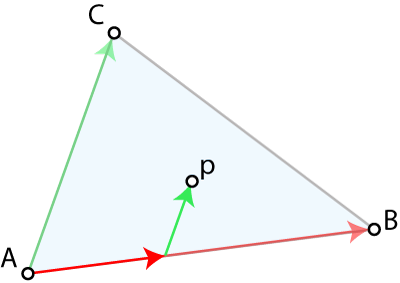
\includegraphics[keepaspectratio,scale=0.5]{barycentric-coordinates.png}
\end{figure}

\par
So, the
$getPosition$
algorithm is as following:

\begin{lstlisting}
R = samplerPointLight.getSample(0)
S = samplerPointLight.getSample(0)
if (R + S >= 1) {
  R = 1 - R
  S = 1 - S
}
x = A.x + R * AB.x + S * AC.x
y = A.y + R * AB.y + S * AC.y
z = A.z + R * AB.z + S * AC.z
return Point3D(x, y, z);
\end{lstlisting}

\par
And the
$intersect$
method is equal to the intersection of a ray with a triangle presented earlier.

\subsection{Cameras}

\par
There was implemented one type of Camera: Perspective Camera.

\par
The camera only provides one method for the user to generate a ray from the camera position in direction to the image plane:

\begin{lstlisting}
Ray generateRay(const float u, const float v,
                const float deviationU, const float deviationV) const;
\end{lstlisting}

\par
The method
$generateRay$
needs four parameters to create a ray.
The $u$ and $v$
are used to choose the pixel in the image plane.
Being
$u$
the inverse of the index of the pixel in its line, that is,
$x / width$
, and
$v$
the inverse of the index of the pixel in its column, that is,
$y / height$.
In order to allow the reduction of aliasing in the generated images of the scene, the camera also accepts two extra parameters
$deviationU$ and $deviationV$
which are variances inside a pixel.
The
$deviationU$
is a horizontal variance of the pixel, that is,
$[-0.5*pixelWidth, 0.5*pixelWidth]$
and
$deviationV$ the variance in the vertical of the pixel
$[-0.5*pixelHeight, 0.5*pixelHeight]$.

\begin{figure}[H]
	\centering
	\caption{Jittering in a plane image.}
	\label{Jittering.}
	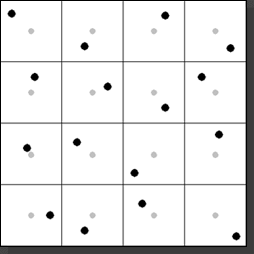
\includegraphics[keepaspectratio,scale=1.0]{Jittering.png}
\end{figure}

\subsubsection{Perspective Camera}

\par
With this type of camera we can simulate images being seen by the human eyes.

\par
To obtain an image plane with perspective is necessary to have a Field of View.
In order to accept any resolution of the image plane, we have to divide the field of view in 2 parts: horizontal and vertical.
This way, we can obtain the aspect ratio of the image plane we want.

\begin{figure}[H]
	\centering
	\caption{Perspective camera with hFov, vFov and dFov.}
	\label{Perspective_Camera.}
	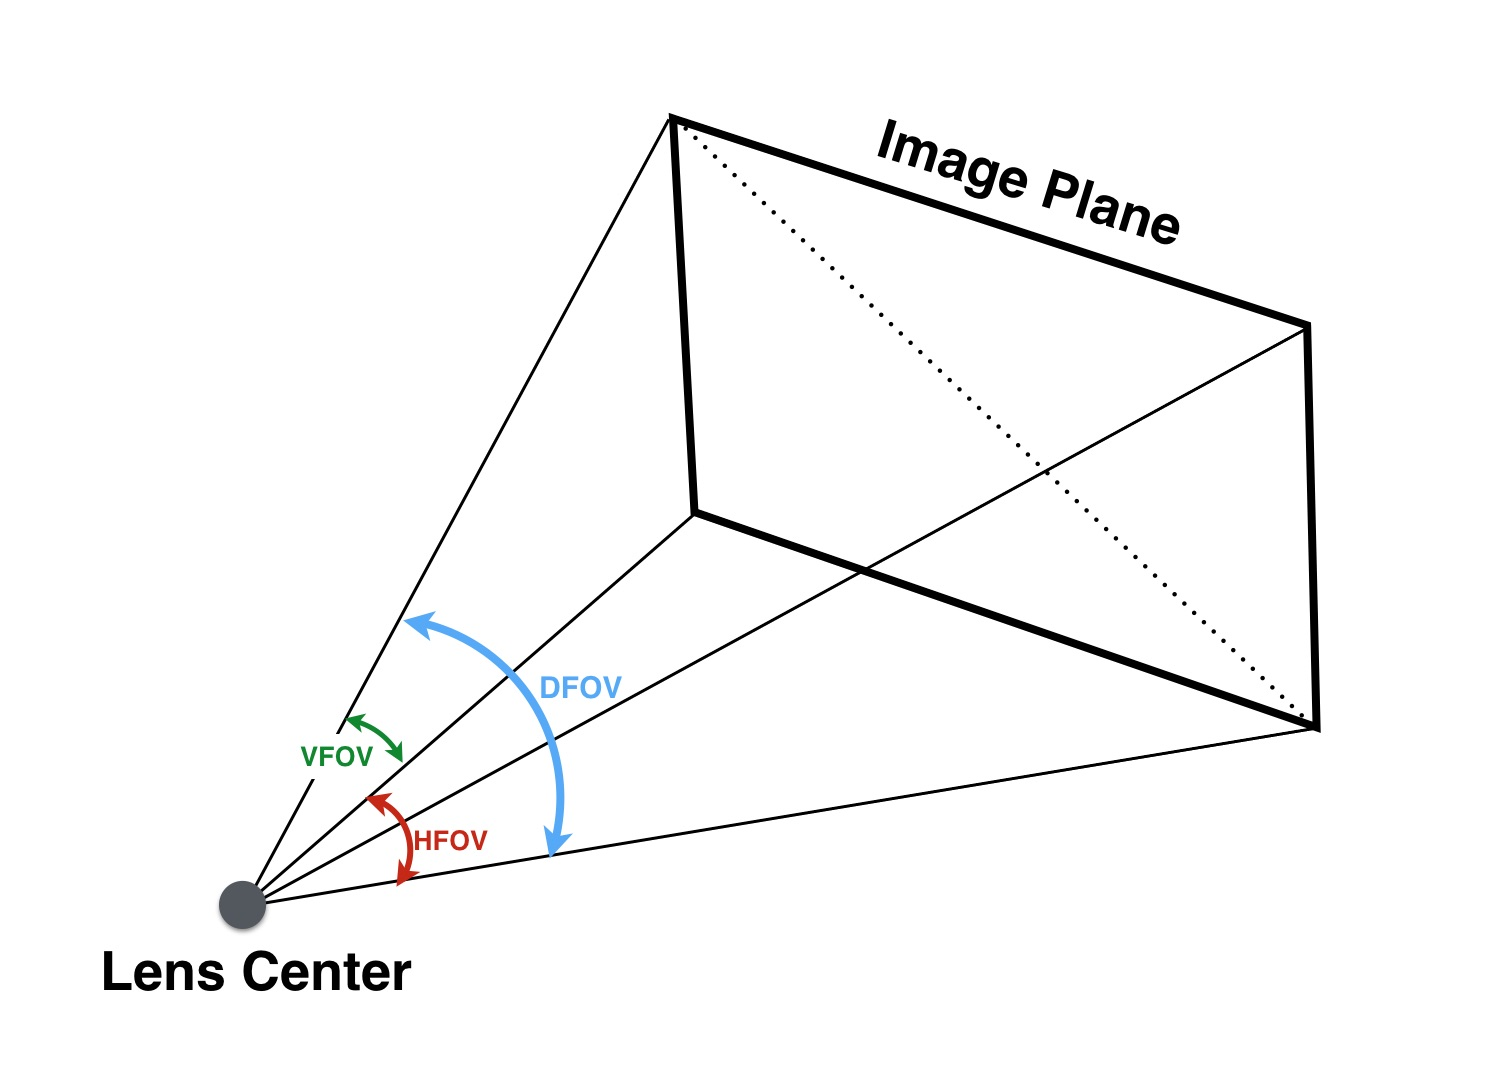
\includegraphics[keepaspectratio,scale=0.2]{hfov-vfov-dfov.jpg}
\end{figure}

\par
The algorithm to generate a ray from the camera is very simple.

...

\section{Android specifics and challenges}

\subsection{Specifics}

\par
Before developing the ray tracer to Android, it is necessary to understand how an Android application works.

\par
A typical Android application is programmed in Java programming language.
And it usually needs to communicate with an User Interface which also is programmed in Java.
The code is compiled with Android Software Development Kit (SDK) along with any data and resource files into an Android package (APK).
But, in order to avoid using the Java Emulator in our code and program it in native code, it is necessary to use Android Native Development Kit (NDK).
Unfortunately, the Android Studio IDE doesn't provide any support like libraries like Qt that facilitates the build of a User Interface in native code.
So, in order to obtain the best performance possible in a mobile device, the User Interface was programmed in Java and the ray tracer library and components were programmed in C++.

\subsection{User Interface}

\par
The Android User Interface is programmed in Java and only one thread can refresh the User Interface (UI thread).

\par
There are only 2 goals about the User Interface: should be as simple as possible and should be able to allow progressive ray tracing (refresh the image while it is being rendered).

\par
In order to allow progressive ray tracing, it was used a pool of 1 thread called Render Task thread that every 200 ms wakes up the thread and updates the strings used in the text view and updates the bitmap of the rendering image by locking and unlocking the pixels.
Locking pixels means that will be ensured that the memory for the pixels will not move until the pixels is unlocked.
Before it finishes, it publishes the progress on the UI thread.
Then the UI thread wakes up and updates the text view.

\begin{figure}[H]
	\centering
	\caption{Execution flow of UI thread and Render Task thread.}
	\label{Execution flow of UI thread and Render Task thread}
	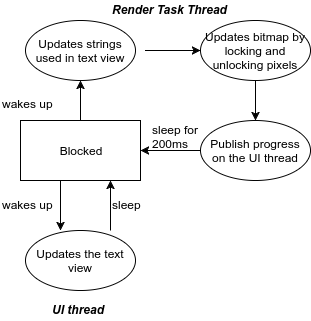
\includegraphics[keepaspectratio,scale=0.5]{UI_thread.png}
\end{figure}

\subsection{Challenges}

\par
Developing applications for mobile devices have different challenges compared with the traditional personal computer hardware.

\par
The Android User Interface has some particularities like only one thread can modify the UI (UI thread).

\par
The memory size is typically lower, the CPU microarchitecture is different and also the Operating System (OS) is shaped for the mobile world, making a lot of restrictions in the performance in order to save battery.
The amount of main memory available for the applications can also be affected by the OS.

\par
Other challenges are related with the communication mechanism between the SDK and the NDK, because two different languages need to “communicate” in runtime (GUI in Java and C++ for the library).
This involves learning how to use the Java Native Interface (JNI), so that both can “communicate” with each other.

\par
Because ray tracing may involve rendering complex scenes, putting all this information in the main memory may not be possible, and so this memory management can be a worthy challenge.

% Chapter - Android -------------------------
% CHAPTER - falar de como uma aplicaçao android funciona
% CHAPTER - falar de como se liga codigo C++ nativo com Java interface
% CHAPTER - falar de cuidados que tive na implementaçao para android
% CHAPTER - falar das possibilidades do android
% CHAPTER - falar das desvantagens do android
\chapter{Demonstration: Global Illumination}

\section{Results obtained}
\label{ResultsObtained}

\par
The developed application ...

\begin{tikzpicture}
\begin{axis}[
legend style={at={(1.05,1.00)},anchor=north west},
axis lines = left,
xlabel = \#threads,
ylabel = speedup,
xtick={0,1,2,3,4},
ytick={0,1,...,10},
]
\addplot [
color=blue,
mark=*,
dashed,
] plot coordinates {
	(0,0.0)
	(1,1.0)
	(2,1.0)
	(3,1.0)
	(4,1.0)
};
\addlegendentry{Without Accelerator Structure}
\addplot [
color=black,
mark=*,
dashed,
] plot coordinates {
	(0,0.0)
	(1,1.0)
	(2,1.0)
	(3,1.0)
	(4,1.0)
};
\addlegendentry{Regular Grid}
\addplot [
color=red,
mark=*,
dashed,
] plot coordinates {
	(0,0.0)
	(1,1.0)
	(2,1.0)
	(3,1.0)
	(4,1.0)
};
\addlegendentry{Octree}
\label{graph:NoShadows}
\end{axis}
\end{tikzpicture}

\section{Comparison with Android CPU Raytracer (\cite{Android_CPU_Raytracer})}

\par
Comparison ...

% Chapter - Conclusion/Future Work --------------
% CHAPTER - dizer que aprendi a fazer um ray tracer do zero
% CHAPTER - dizer que aprendi a fazer uma aplicaçao android
% CHAPTER - falar de possiveis componentes/estruturas de aceleraçao a implementar
% Tentar chegar às 50 páginas antes do capítulo 5
\chapter{Conclusion \& Future work}

\section{Conclusions}

\par
The constant evolution of technology allowed to leverage and massify the mobile devices.
With more and increasingly powerful mobile devices, it is possible to perform more and more complex and useful tasks in them.
This is a huge market where the programmers can develop their applications to and where the development time can be a huge factor in their career success.

\par
But as noted in this pre-dissertation report, there is clearly a lack of well documented rendering libraries for mobile systems.
There is then the need to change this reality, since more and more the Internet of Things is more present each passing year, because there are increasingly powerful mobile systems.

\par
As it is possible to address a huge number of challenges while developing the ray tracer, this pre-dissertation identified some of the strategic decisions to be performed in this dissertation project and its related challenges that may arise during the development.

\section{Future Work}

\par
With respect to future work, it should be the development of the library for Android and the analysis of possibilities and challenges that may arise.
Upon completion of the development process, besides writing the dissertation and the article, it is expected to provide a demo application in order to illustrate the functionalities and performance that the library will offer.

%- Bibliography (needs bibtex) -%
\bibliography{dissertation}
\nocite {*}

\begin{appendices}
\chapter{User documentation}
\end{appendices}

\end{document}